
\section{Dynamics}
\label{sec:dynamics}
Our method extends trivially to dynamic simulations that include inertial
effects. However, it is important to note that the indefiniteness encountered in
quasistatic time stepping also arises in implicit time stepping for
dynamics. Fortunately, the definiteness fix outlined above can be used in this
setting as well. \oldtext{Here we will outline why this indefiniteness is
  increasingly likely to occur when performing interactive high-resolution
  simulation.} In this case, we typically desire a fixed, \oldtext{temporal
  resolution}\newtext{large time step} of
$\Delta{t}\approx\frac{1}{30}$. Using \oldtext{the common} backward Euler
time stepping scheme \oldtext{for illustration,}
and \newtext{a}\oldtext{assuming that the resulting non-linear equations are solved with}
Newton-Raphson \newtext{linearization}, the following \newtext{linear} update equation must be solved for the increment $\delta\vec{{x}}$ in the $k^\textrm{th}$ iteration
% To demonstrate this fact, let us examine the comparatively simple case of backward Euler time stepping. Here, our discrete system of equations is:
% $$
% \frac{\vec{x}^{n+1}-\vec{x}^{n}}{\Delta{t}} = \vec{v}^{n+1}\ \ \mbox{and}\ \ 
% \mathbf{M}\left(\frac{\vec{v}^{n+1}-\vec{v}^{n}}{\Delta{t}}\right) = \vec{f}(\vec{x}^{n+1})
% $$
% where $\mathbf{M}$ is the mass matrix associated with the material of interest. 
% %
% % For example, in a finite element based discretization one would use $M_{ij}=\int_{\Omega_0}{\rho(\mathbf{X})}{N_i}{N_j}d\mathbf{X}$ where $N_i$ and $N_j$ are the interpolating functions associated with each degree of freedom and $\rho$ is the mass density of the material. However, in graphics it is common to use a diagonal approximation (or mass lumping approximation) to this matrix obtained by summing each row: $M^\textrm{d}_{ii}=\sum_jM_{ij}$. This is equivalent to assigning each node an equal portion of volume of each of its incident elements and then determining the mass of the node as density times this volume. For example, in a tetrahedron based approximation each node would be given one fourth of the volume of each of its incident tetrahedra. 
% %
% We can solve this non-linear system by first eliminating $\vec{v}^{n+1}$ to get
% $$
% \mathbf{M}\left(\vec{x}^{n+1}-\vec{x}^{n}\right) = \Delta{t}\mathbf{M}\vec{v}^n + \Delta{t}^2\vec{f}(\vec{x}^{n+1})
% %\mathbf{M}\left(\frac{\frac{\vec{x}^{n+1}-\vec{x}^{n}}{\Delta{t}}-\vec{v}^{n}}{\Delta{t}}\right)=\vec{f}(\vec{x}^{n+1})
% $$
% and then performing Newton iteration for $\vec{x}^{n+1}$. At the $k^\textrm{th}$ Newton iteration, we update an approximation to $\vec{x}^{n+1}$ given by $\vec{x}^{n+1}_{k+1}= \vec{x}^{n+1}_{k}+ \vec{\delta{x}}$ by solving the system
$$
\mathbf{K}^\textrm{BE}(\vec{x}^{n+1}_{k}) \delta\vec{{x}}=\Delta{t}\mathbf{M} \vec{v}^n+\Delta{t}^2 \vec{f}(\vec{x}^{n+1}_{k})
$$
Here $\mathbf{K}^\textrm{BE} =
\mathbf{M}+\Delta{t}^2\mathbf{K}(\vec{x}^{n+1}_{k})$, and $\mathbf{M}$ is the
mass matrix. \oldtext{The i}\newtext{I}ndefiniteness of $\mathbf{K}(\vec{x}^{n+1}_{k})$ can
thus be seen to potentially cause indefiniteness of \oldtext{the
  backward Euler system matrix
}$\mathbf{K}^\textrm{BE}(\vec{x}^{n+1}_{k})$. \newtext{One could attempt to manipulate
  nodal masses or material properties to preserve definiteness, but this alters the
  behavior of the simulation in arbitrary ways.}
\oldtext{Specifically, there are three factors that will conspire to yield
  indefiniteness in the  backward Euler system matrix: time step size
  ($\Delta{t}$), nodal mass ($M_{ii}$) and relative magnitude of elasticity
  parameters ($\mu$,$\lambda$). It may be tempting to adjust these parameters to
  provide a definite backward Euler system matrix. For example larger nodal
  mass, smaller $\Delta{t}$ and smaller $\mu,\lambda$ have a better chance of
  yielding a definite matrix. However, altering the nodal mass or elasticity
  coefficients would be equivalent to altering the behavior of the material
  inherent in the governing equations and should therefore be considered off
  limits.} \newtext{Although decreasing the timestep could also fix
  the indefiniteness, } \oldtext{when interactivity is desired} the
time step cannot be decreased arbitrarily \newtext{when interactivity is desired}.
Furthermore, it is important to note that the nodal mass is proportionate to the
volume associated with each node. Therefore, as we increase the discrete spatial
resolution of our domain, the nodal mass decreases thereby increasing the
likelihood of encountering an indefinite backward Euler system matrix as it
would behave more and more like the indefinite $\mathbf{K}(\vec{x}^{n+1}_{k})$
\newtext{(see Figure} \ref{fig:evalues} \newtext{for a numerical experiment that
  demonstrates this behavior)}. Therefore, \oldtext{we see that} when
\oldtext{maximum}\newtext{both high} performance
and high resolution are desired, indefiniteness in the backward Euler system
matrix \oldtext{is a distinct possibility}\newtext{quite likely}. Fortunately, the definiteness fix
\oldtext{outline above}\newtext{in section~{{\ref{sec:indefiniteness}}}} for $\mathbf{K}(\vec{x}^{n+1}_{k})$ \oldtext{suffices to }guarantee\newtext{s} definiteness of the backward Euler system matrix.
\vspace{-10pt}
\begin{figure}[h]
\center{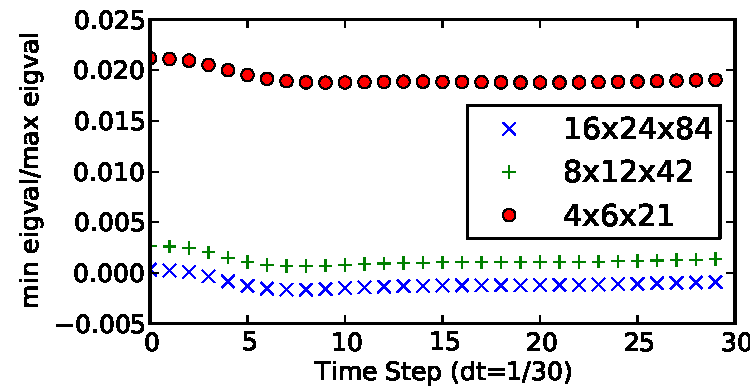
\includegraphics[width=\columnwidth]{elasticity/figures/evalue_plot}}
\vspace{-15pt}
\caption{\newtext{Plot of ratios of minimum to maximum eigenvalues of the
    backward Euler matrix of a dynamic elastic bar simulation without our
    definiteness fix applied. Note that the minimum eigenvalues are negative in the
    16x24x84 resolution example.}}


%Ratio of min to max eigenvalue at each time step of a dynamic
%    elastic bar simulation at various resolutions with no definiteness fix.. These are the eigenvalues that would arise without the definiteness fix of the backward Euler matrix. Note that the minimum eigenvalues for the highest resolution are substantially negative.}}
\label{fig:evalues}
\vspace{-10pt}
\end{figure}
